The implementation will consist of three parts. The server, The device in the users home used to 
collect and send usage data, and the Android application. The android application is the main focus for 
this project and most of the teams resources will be used on this.

\subsubsection{Server}
The server will consist of two parts. One for handling requests from the Android application and one for storing data that is collected in the users home. 
The part that handles the android application will be running Dropwizard~\cite{dropwizard} which is a collection of Java libraries that together make a REST service. 

These libraries include Jetty~\cite{jetty}, Jersey~\cite{jersey}, JDBC~\cite{jdbc}, and Jackson~\cite{jackson}. The server will expose a set of URL's that will provide the android application with 
possibilities to get and store data from the database. The other part, that stores data from the users home is under development.

\subsubsection{Android Device}
The application running on the users Android device will be designed to run on Android 4.0 or greater.
The team will also use the Model-View-Presenter (MVP)~\cite{mvp} this is a Model-View-Controller (MVC)~\cite{mvc} derivative 
that pushes almost all logic into the presenter. The application will follow standard Android design guidelines~\cite{androidgui}
when it comes to user interface design.

\subsubsection{Home Data Aggregator}
This device will collect data from sources in the user's home. The reason for this external box as opposed to using 
the user's phone to collect data, is that with this solution the system can fetch data at regular intervals throughout 
the whole day. This would result in that the user would not need to be home in order for the application to collect 
usage data. The device will pass data along to the external server at request from the server.

\begin{figure}[H]
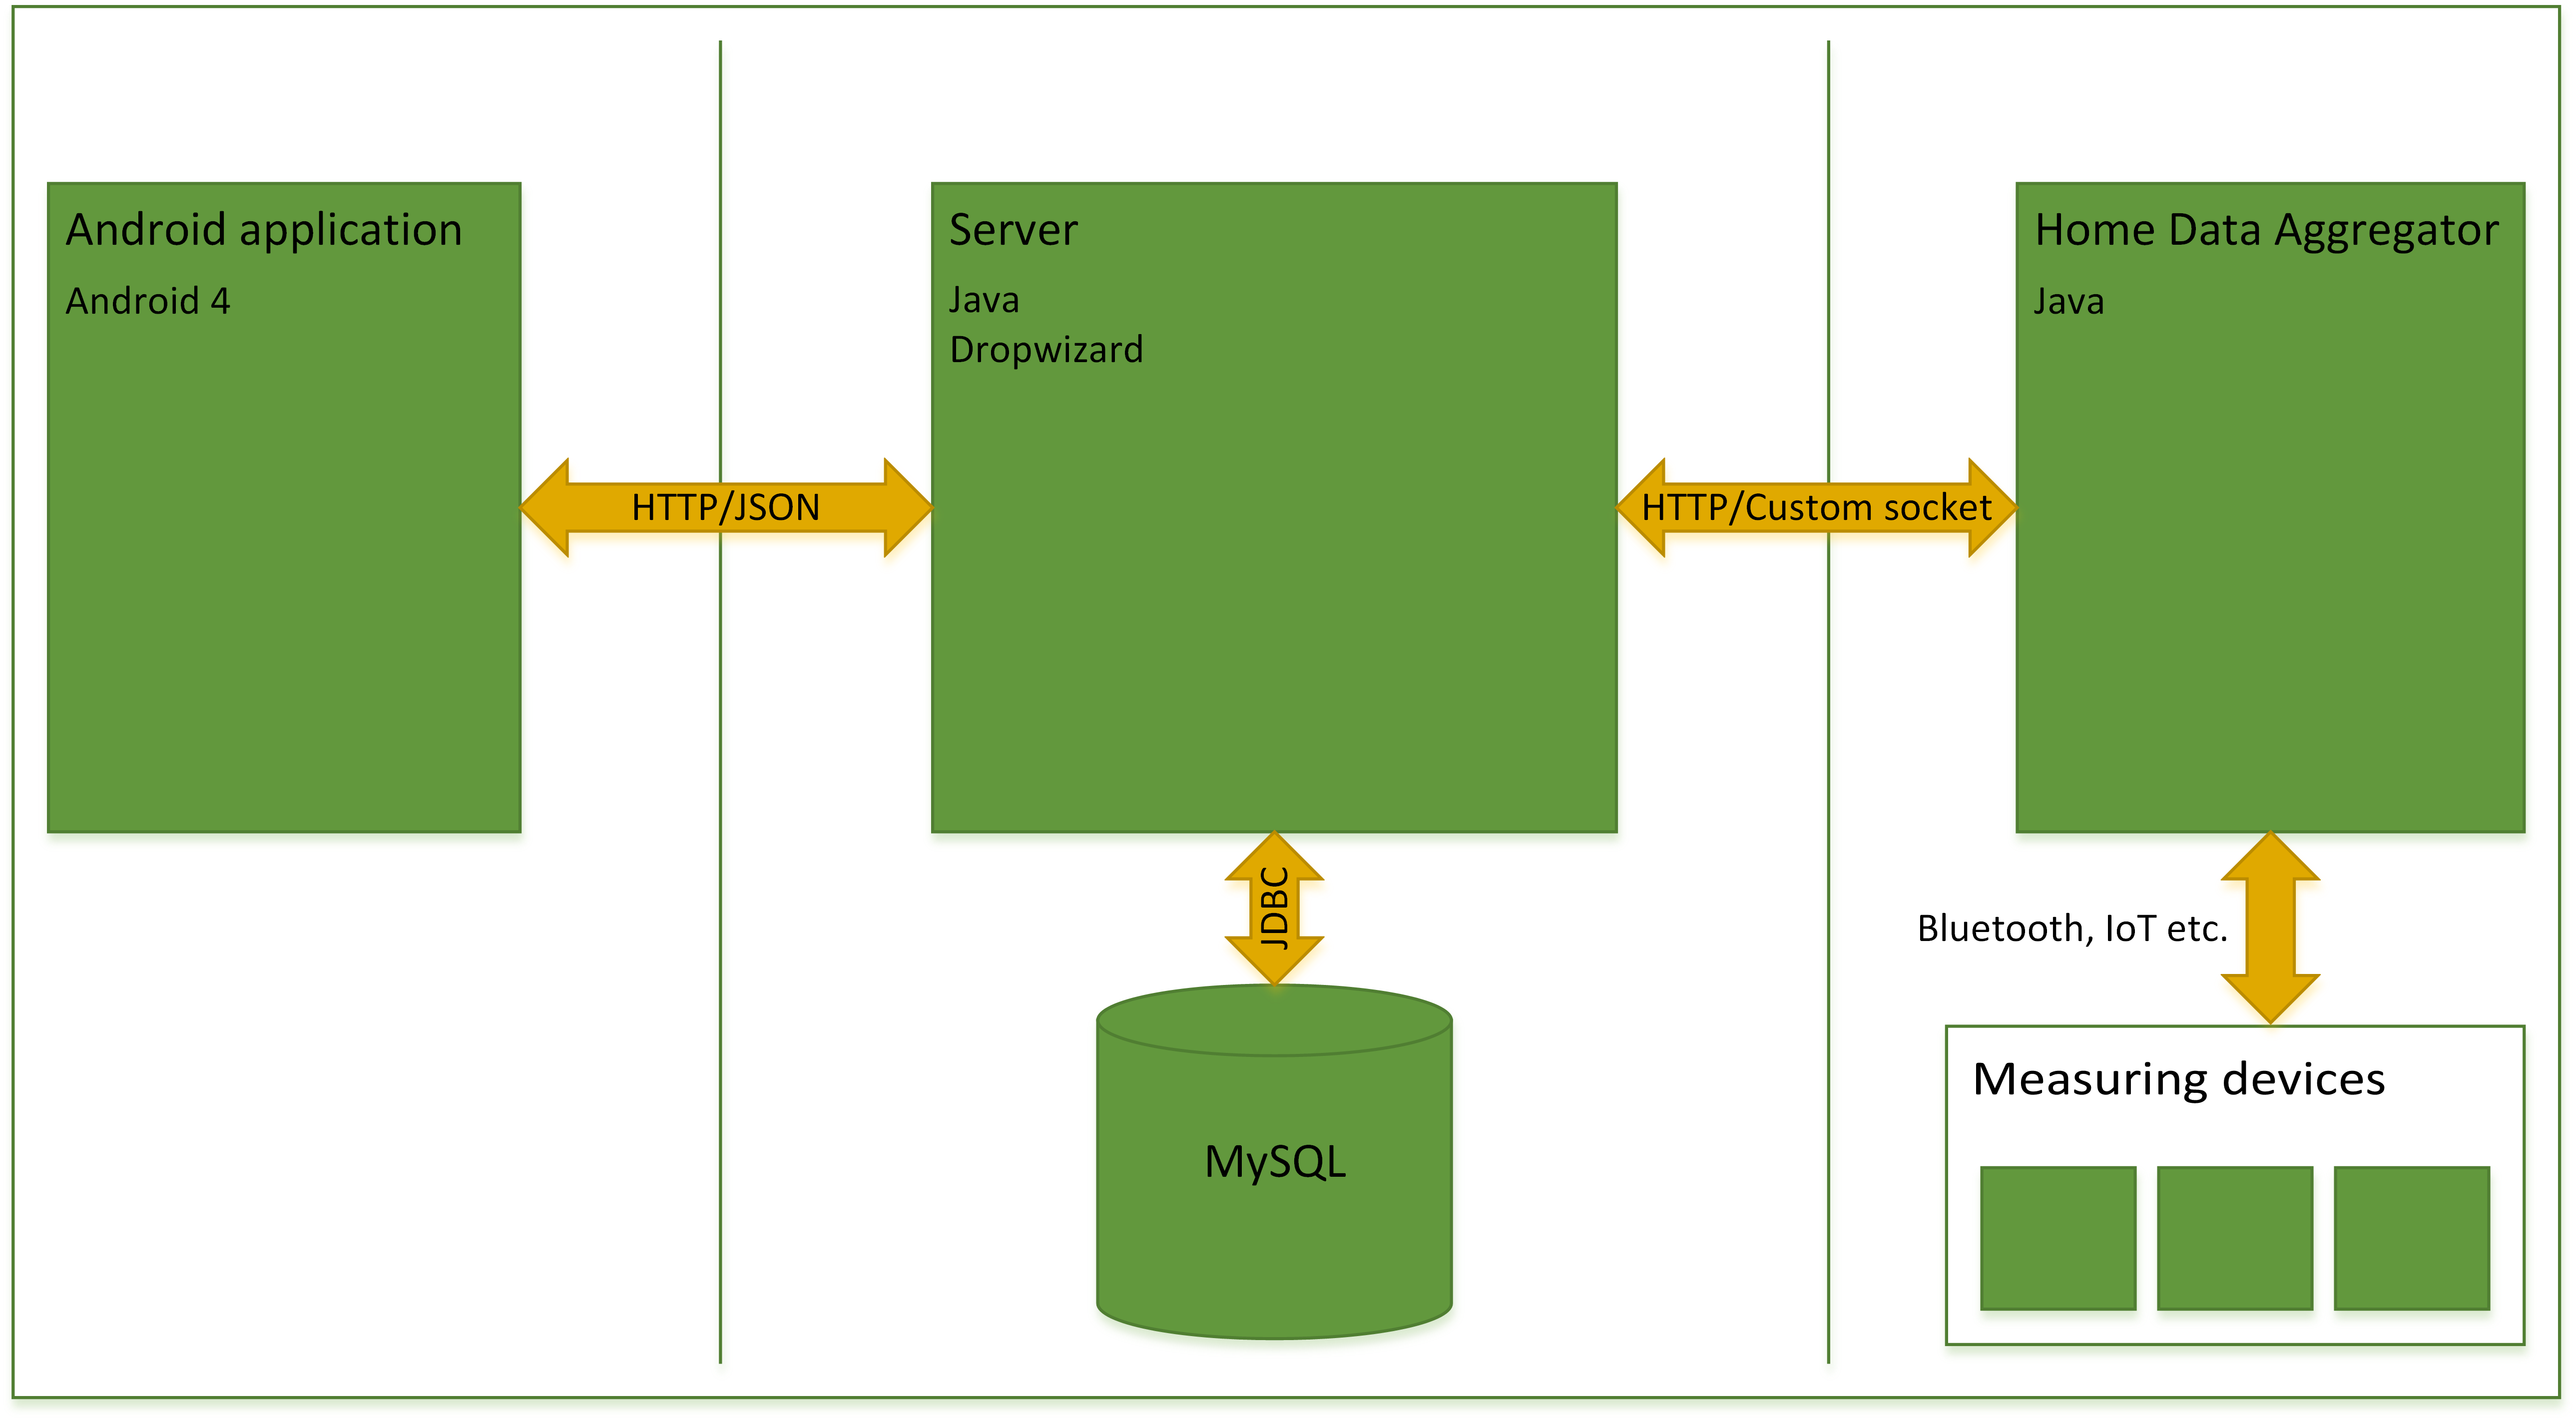
\includegraphics[width=\textwidth]{ch/implementation/fig/architecture.png}
\caption{Architecture}
\end{figure}